\documentclass[12pt]{article}
\usepackage{graphicx}
\usepackage[letterpaper]{geometry}
\usepackage{times}
\geometry{top=1.0in, bottom=1.0in, left=1.0in, right=1.0in}

\usepackage{setspace}
\doublespacing

\usepackage{fancyhdr}
\pagestyle{fancy}

\lhead{}
\chead{}
\rhead{Petroff, Cao \thepage}
\lfoot{}
\cfoot{}
\rfoot{}
\renewcommand{\headrulewidth}{0pt}
\renewcommand{\footrulewidth}{0pt}

\setlength\headsep{0.333in}

\newcommand{\bibent}{\noindent \hangindent 40pt}
\newenvironment{workscited}{\newpage \begin{center} Works Cited \end{center}}{\newpage }

\begin{document}
\begin{flushleft}
Zachary Petroff, Kevin Cao \\
Professor Rodriguez \\
Introduction to Artificial Intelligence \\
26 April 2020

\begin{center}
\textbf[Grocery Run Game]

Using a Genetic Algorithm to Train Perceptrons on Navigating Obstacles
\end{center}

\setlength{\parindent}{0.5in}
\noindent\textbf{Problem Space}

The game is fairly simple. The player plays the role of a shopping cart and can choose to jump, do nothing, or crouch. Obstacles will scroll across the screen, and the player has to choose to either jump over the obstacle, crouch underneath, or just do nothing. As the game progresses, the obstacles move faster and faster, increasing the difficulty of the game. The objective is to last as long as possible, as the time elapsed is equal to the score.
For a simple game like this, it would be trivial to create an algorithm that could simply read the distance between the next obstacle and the player, the type of obstacle, and calculate the precise moment in which to jump. However, this approach did not seem to be in the spirit of artificial intelligence, so we chose to use a genetic algorithm to do so. With that in mind, there were a couple of obstacles to approach. What sort of data should we provide the algorithm? Including too much detail about the game would slow the algorithm down, but leaving too much out would result in little to no progress per generation. In addition, what exactly would the algorithm be training? What sort of data structures would we use as input to the algorithm? These were the main problems we had to tackle.

Other variations of this game would mostly be more complex, difficult versions of the game. 3D variations would be a far more interesting game to implement the genetic algorithm for, due to complexities that adding another dimension introduces. Another variant could possibly be maze games, although the main difference is that instead of simply avoiding obstacles, the player must also consider \emph{how} the obstacle should be maneuvered.

\hfill

\noindent\textbf{Algorithms}

\noindent\emph{Basic Perceptron}


There were two networks used to train the player: a basic perceptron and a multilayer perceptron. The basic perceptron consists of three inputs, three weights, three biases, and a threshold. The inputs to the perceptron, in this case, are the current speed of the runner, the distance from the next goal, and the Y position of the obstacle. If the dot product of the inputs and the weights, plus the sum of biases, reach the threshold, then an action is produced. Otherwise, the player stays on the ground and keeps moving forward until the threshold is reached. 

\hfill

\noindent\emph{Multilayer Perceptron}

The multilayer perceptron has the same inputs; however, there are six weights that need training. Like in the basic perceptron, the dot product of the inputs and weights is found. However, instead of having a threshold, this unit is connected to three output nodes, each with their own weight. These nodes correspond to three possible actions the player could take: jump, crouch, or do neither. The softmax probability distribution of these nodes is then found, and the highest probability is chosen. 

\hfill

\noindent\emph{Genetic Algorithm}

Each of the parameters were found using a genetic algorithm. To train the genetic algorithm, a random population of genotypes, each with the appropriate amount of bits, is initially created. Each of the bits represent a parameter in the network that has to be trained. To train the network, two genotypes from the population are chosen at random, and made to compete against each other, through the use of a fitness function. The fitness function used simply returns the score obtained by the genotype after playing the game. The loser is then mutated and recombined. The mutation function iterates through each bit in the losing genotype, with each bit having a chance (based on the mutation probability previously set) of having a random value added to it. The recombination function is very similar, however, instead of adding a random value to the bit, it completely replaces that bit with the corresponding bit from the winning genotype. Overtime, the network is able to find better solutions, until it seems that the network is unable to learn any further.

\hfill

\noindent\textbf{Drawing Parallels Between Computation and Brain}

\noindent\emph{The Similarities Between a Perceptron and a Biological Neuron}

Like a perceptron, a biological neuron has a threshold that fires if and only if that threshold is reached. However, in a neuron, the distance from the threshold is much more dynamic. For a perceptron, the distance is decided by the inputs, but in a neuron, there might be an influx of sodium, an outflux of potassium, or the firing of a presynaptic neuron that all influence whether an action potential is fired. While both a perceptron and a neuron act on the all-or-none principle, in a perceptron, the influences governing whether or not an action potential is reached are much more transparent. 

Moreover, in a perceptron, there are weights that can be thought of as a measure of synaptic strength between neurons. The synaptic strength between neurons refers how much a presynaptic neuron firing influences the membrane potential of a postsynaptic neuron. The greater the synaptic weight, the more likely the postsynaptic neuron will fire as a result of the presynaptic neuron firing. Just as, in a perceptron, the greater the weight between an input node and an output node, the greater effect the input will have in reaching the threshold. However, due to the method of training (a genetic algorithm), the synaptic weights are chosen randomly and allowed to continue on if they produce the desired behavior. While, between neurons, synaptic strength is increased by a process called long-term potentiation, that occurs if the pre- and postsynaptic neurons fire at the same time.

\hfill

\noindent\emph{The Similarities Between Softmax and Lateral Inhibition}

Lateral inhibition occurs when an activated neuron reduces the activity of its neighbors (Bailey). Similarly, if we look at each of the output nodes when using the softmax activation function as neurons, if one neuron fires, this means that the rest of the neurons are inhibited and unable to fire. However, there are differences between lateral inhibition and softmax. In lateral inhibition, the activation of neighboring neurons merely reduces activation, while softmax completely suppresses all other neurons. Furthermore, when using the softmax, all neurons besides the one being activated are suppressed, meaning there is no correlation between suppression and distance from the activated neuron like in lateral inhibition. 

\hfill

\noindent\textbf{Empirical Analysis}

The following results were from running the AI for multiple generations, and tracking the average score (time spent alive) over the entirety of each generation.

In the following set of data, there were only obstacles the agent needed to jump over. There were no obstacles in which the agent should not jump. Two separate runs were recorded, and the genetic algorithm started from scratch each time. The X axis represents each generation. 

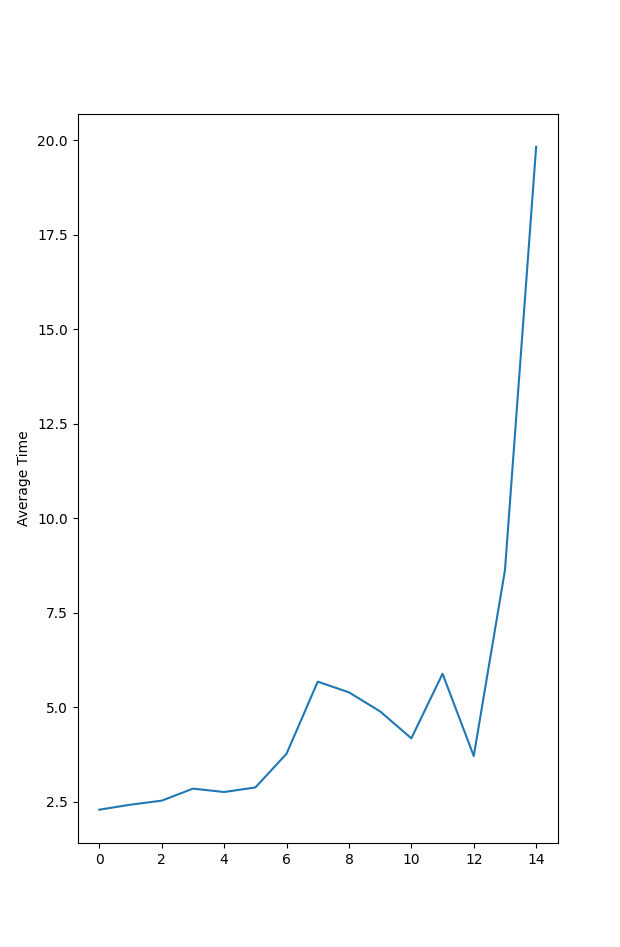
\includegraphics[scale=.4]{Figure_1.png}
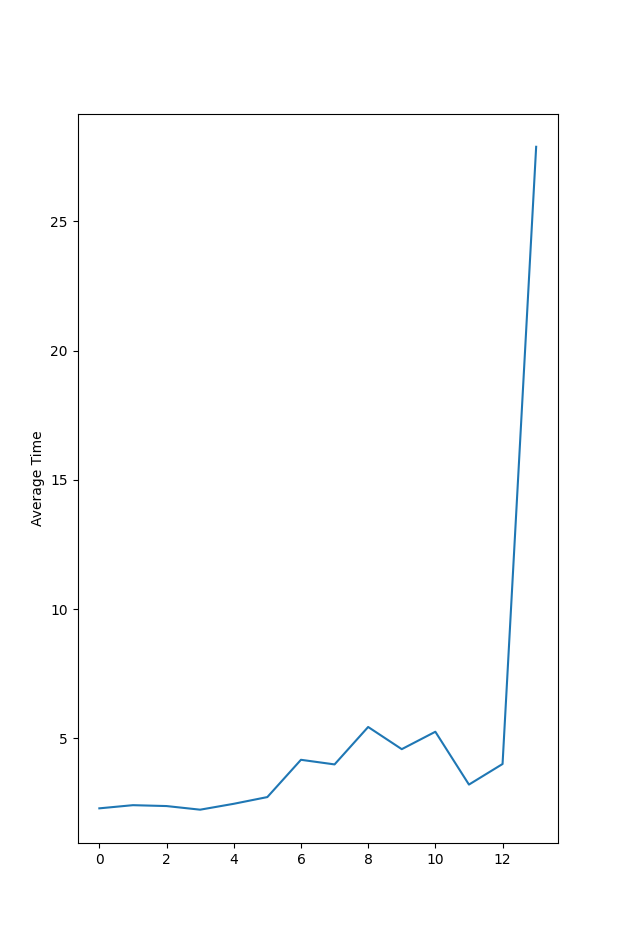
\includegraphics[scale=.4]{Figure_2.png}

Notably, there is certainly an increase in performance, with spikes at around generation 5, and a significant jump at around generation 13. After generation 14, we would reach an agent that would not lose (tests were stopped once an agent survived for 10 minutes straight).

We certainly expected an improvement as demonstrated, but did not expect a ``perfect" player at such an early generation. Such quick improvement implies that the problem space is not particularly different for the AI to navigate.

\hfill

To further challenge the AI, we then included flying obstacles, but only ones that the agent should not jump over. Attempting to jump over the flying obstacle would result in a collision, but simply doing nothing would allow the player to pass right underneath. We expected this to result in much slower progress in learning as this would add another layer of decision-making rather than simply ``jump at every obstacle".

Surprisingly, this did not affect the progress at all, and in some cases, would actually result in a ``perfect" player earlier, as demonstrated in the following graphs:

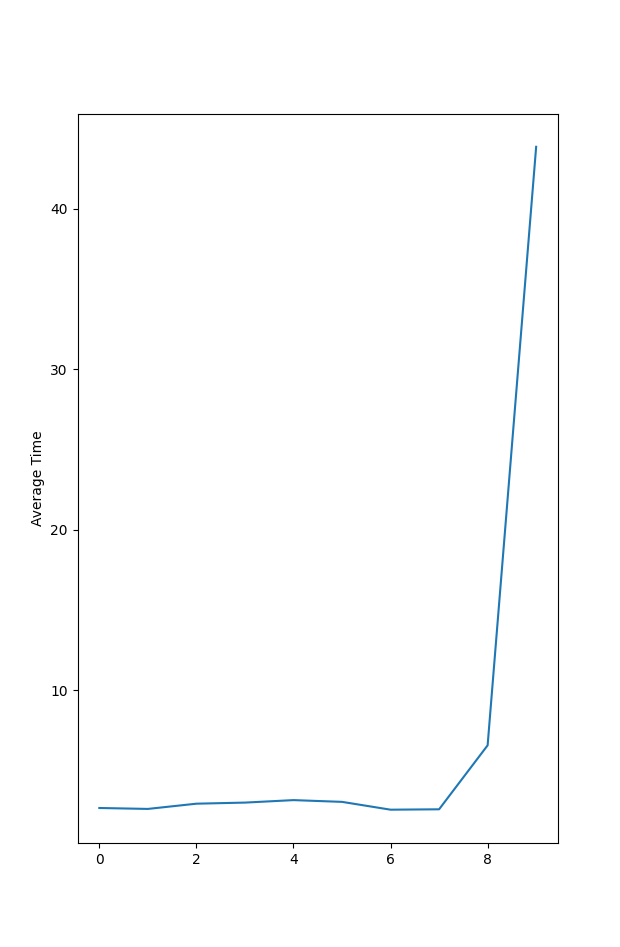
\includegraphics[scale=.4]{Figure_4.png}
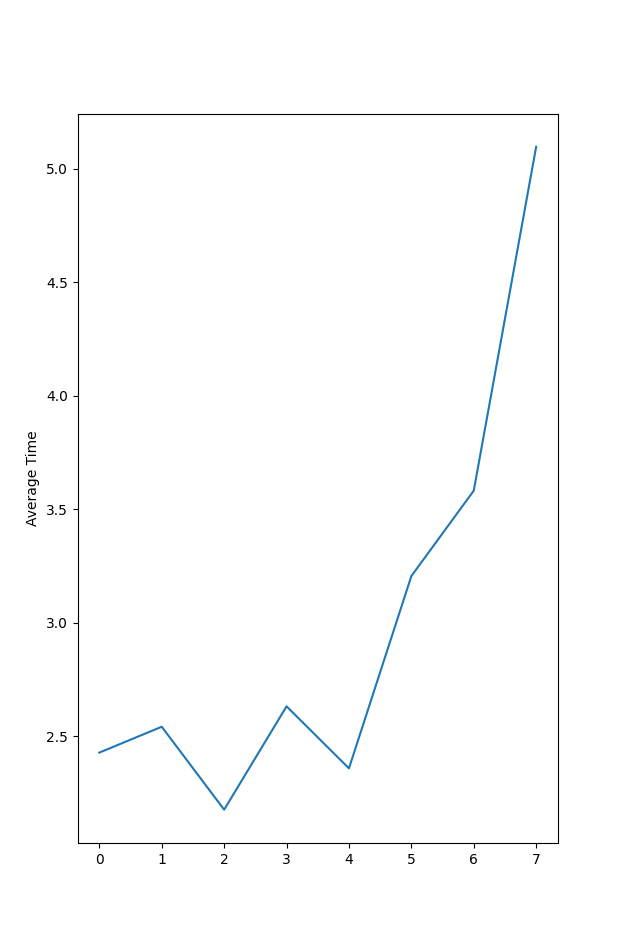
\includegraphics[scale=.4]{Figure_5.png}

We can see that despite the addition of a new obstacle, the player reaches ``perfection" at around generation 7. This sort of pattern implies that perhaps adding these new obstacles to the problem space without adding a new behaviour to the AI (e.g. crouching), does not necessarily mean that progress will be slowed.

Unfortunately, at the time of this report, the implementation for a multi-layer perception that allows for crouching has not been completed, so we do not have the data to truly see what would happen if we implement a new behavior.

\hfill

\noindent\textbf{Ways to Improve Performance}

\noindent\emph{A Better Network Structure}

One way to improve the performance of our network is by changing the structure. Currently, the most complex network has only one hidden layer. By increasing the number of layers, presumably the network would be able to learn more complex behaviors to improve performance. This is because the network would have the opportunity to use additional nonlinear functions. The use of more nonlinear functions may allow the network to draw a more accurate decision boundary. 
Moreover, the number of inputs in the input layer could be increased to produce a similar  result. Currently, our networks take in the current speed of the player, the distance from the next obstacle, and the Y position of that obstacle. Presumably, the speed and distance allow the network to discern the time it will take to reach the obstacle, while the Y position conveys to the network whether the obstacle will be on the ground or in the air. However, additional information might be of use to the network. For example, the current acceleration may be of use when deciding precisely when to jump or crouch. Another example may be the size of the obstacle. If the network was in a position where it knew to jump, but did not know the duration of the jump, the game might end with the player clipping the back of the obstacle. 
  However, by increasing the number of hidden layers and/or inputs, the training time is also increased. This is because the genetic algorithm would have to search for more weights. To find any given weight, the genetic algorithm might have to test over a hundred different genotypes. Moreover, calculating the values at each of the additional layers/inputs would also increase training time. So, while the network may be able to learn more given more layers and inputs, there is a downside. Certainly, if we measured the behavior of the network as the number of layers and inputs are increased, there would be a plateau of performance at some point. At this point, no longer would the increased training time be worth slightly increasing the performance.

\hfill

\noindent\emph{A Better Training Method}

Because genetic algorithms are subject to randomness, an improvement would be a more precise method of training. There exist many different methods, however, reinforcement learning seems to be the most effective when trying to teach a network how to play a game. There are many famous examples in the history of Artificial Intelligence that display the proficiency of reinforcement networks, such as DeepBlue and AlphaGo. 
Reinforcement networks learn by providing the player with a reward or punishment corresponding to each of its actions. With each iteration, the player is enticed to produce good behavior, while at the same time being cattle-prodded away from undesired behavior. This proves to produce unmatched results, and is more precise than the guess-and-check method used by a genetic algorithm. To explain exactly why this is desirable, consider the problem of trying to train an agent to navigate to the top of a mountain. A genetic algorithm might get lucky and produce an outcome that allows the agent to get very close to the top. However, the time it would take to find a better outcome is completely unknown. The genetic algorithm might explore thousands of worse solutions before it finds a better one. With reinforcement learning, on the other hand, the network could incrementally find better solutions, until it reaches the top. In other words, we know roughly how long the training would have to take place and how well our network could do. 

\begin{workscited}
\thispagestyle{plain}
\bibent
  Bailey, Regina. “Lateral Inhibition: Neuron Suppression Enhances Sensory Perception.” \emph{ThoughtCo}, ThoughtCo, 30 June 2019, www.thoughtco.com/lateral-inhibition-4687368.

\end{workscited}
\end{flushleft}
\end{document}
